\chapter{القوانين الثابتة، والمتجهات الرباعية، وموتر المجال}

سنبدأ بقانون كان يمكن للطبيعة أن تمتثل له، لكنها لا تفعل. وسيكشف لنا إخفاقه كيف ينبغي أن يُكتب القانون الفيزيائي. والاختبار نفسه يقود أولًا من مركبات الإحداثيات إلى المتجهات العادية، ثم من المتجهات العادية إلى المتجهات الرباعية، وأخيرًا من المتجهات الرباعية إلى الموترات. وبحلول النهاية، لن يعود المجالان الكهربائي والمغناطيسي جسمين منفصلين: بل سيشغلان معًا الخانات الست المستقلة لموتر واحد متضاد التناظر.

ما لم يُذكر خلاف ذلك، نستخدم وحدات يكون فيها \(c=1\)، ونرتب مركبات الزمكان على النحو \((1,2,3,0)=(x,y,z,t)\)، ونستخدم اصطلاح إشارة المترية \((-,-,-,+)\).

\section{قانون ممكن ذو تناظر خاطئ}

ثبّت محورًا \(x\) ومحورًا \(y\) تثبيتًا دائمًا في الفضاء. ولنفرض الآن أن جسيمين يتفاعلان كلما تساوت إحداثياتهما \(x\). قد يعكس التفاعل حركتهما أو يرسلهما مبتعدين في اتجاهات جديدة؛ وديناميكا هذا التفاعل التفصيلية لا تهم. وشرط البدء المقترح هو ببساطة \begin{equation}
  x_1-x_2=0,
\end{equation} حيث تشير الرموز السفلية إلى الجسيمات لا إلى مركبات الإحداثيات. ولا يوجد في هذه القاعدة أي تناقض رياضي. والسؤال هو: ما الذي يجعلها غير معقولة فيزيائيًا؟

\begin{classroomqa} \audiencequestion{هل تنتهك هذه القاعدة تجانس الفضاء؟} \lecturerresponse{لا. إن نقل المبدأ يغيّر الإحداثيين بالمقدار نفسه ويترك \(x_1-x_2\) دون تغيير. ولا تحدد هذه القاعدة أي موضع مفضّل. أما عيبها فهو تماثل الخواص في جميع الاتجاهات: فهي تميّز اتجاهًا مفضّلًا واحدًا.} \end{classroomqa}

أدِر المحاور بزاوية \(90^\circ\). فالجهة القديمة \(x\) تُسمّى الآن \(y\)، ولذلك ستوصَف الأحداث الفيزيائية نفسها بتساوي الإحداثيين \(y\). وعند زاوية عامة سيدخل في الشرط تركيب خطي من \(x\) و\(y\). ولذلك تعتمد صيغة القانون على الكيفية التي وُجّهت بها السبورة. فهو ثابت تحت الإزاحة، لكنه غير ثابت تحت الدوران.

نعطي القوانين الفيزيائية عادة أبسط صورها في إحداثيات متعامدة. ويمكن استعمال إحداثيات أكثر عمومية، لكن المترية والصيغ تصبحان عندئذ أقل بساطة. وضمن فئة الأطر الديكارتية المتعامدة، لا ينبغي تمييز أي توجّه.

والإصلاح فوري. ففي بُعدين نطلب تساوي الإحداثيين كليهما؛ وفي ثلاثة أبعاد نطلب تساوي الإحداثيات الثلاث كلها: \begin{equation}
  x_1=x_2,
  \qquad y_1=y_2,
  \qquad z_1=z_2.
\end{equation} وعندئذ لا يمكن للجسيمين أن يتفاعلا إلا عندما يبلغان النقطة نفسها، حتى لو اقتربا منها على امتداد خطين مختلفين.

\begin{classroomqa} \audiencequestion{وهل يجب أن تتساوى أيضًا إحداثيات \(z\) والأزمنة؟} \lecturerresponse{في الفضاء الثلاثي الأبعاد يجب أن تتساوى أيضًا إحداثيات \(z\). ويُغفَل الزمن في الوقت الراهن؛ وسيُعاد إدخاله ما إن يكتمل البرهان المكاني.} \end{classroomqa}

لتكن \(\boldsymbol r_a\) موضع الجسيم \(a\). تصبح شروط المركبات الثلاثة معادلة متجهية واحدة، \begin{equation}
  \boldsymbol r_1-\boldsymbol r_2=\boldsymbol 0.
\end{equation} قد تنعدم مركبة في إطار مُدار ما، ولا تنعدم في إطار مُدار آخر. أما المتجه كله فالأمر مختلف: فإذا كانت كل مركبة فيه صفرًا في إطار ما، كانت كل مركبة فيه صفرًا في كل إطار مُدار. وكذلك إذا كان متجهان متساويين في إطار ما، فإنهما يظلان متساويين بعد تحويلهما معًا.

\begin{figure}[H] \centering
\includegraphics[width=0.78\textwidth]{lecture_06_figure_01.png} \caption{تساوي الإحداثيات الثلاثة الذي يجعل التصادم يعني التطابق المكاني بدلًا من التطابق على طول محور مفضّل واحد.} \lectureframe{00:09:00} \end{figure}

ولهذا تكون المعادلات المتجهية مفيدة. فمركباتها تتغير، لكن الكمية نفسها تتحول على نحو متسق. ويمكن لقانون يُكتب للكمية الكاملة أن يحتفظ بصيغته عندما تُدار الإحداثيات.

\section{التطابق في الزمكان}

استبدل الآن المحور المكاني الرأسي بالزمن. فقد تقول قاعدة نيوتونية إن تغيرين في الحركة لا يحدثان إلا عند أزمنة متساوية. ففي الميكانيكا النيوتونية يكون التزامن مشتركًا بين جميع المراقبين العطاليين، ولذلك تكون مثل هذه القاعدة ممكنة. أما في النسبية الخاصة فإنها تنتقي إطارًا مفضّلًا. فالأحداث المتزامنة في إطار ما لا يلزم أن تكون متزامنة في إطار آخر.

وليس اشتراط تساوي الإحداثيات المكانية وحدها أفضل حالًا. فقد تكون لإزاحة زمكانية مركبات مكانية منعدمة ومركبة زمنية غير منعدمة، \begin{equation}
  \Delta X^\mu=(0,0,0,\Delta t),
\end{equation} ويخلط التعزيز \(\Delta t\) بمركبة مكانية. والعبارة المحلية الثابتة هي أن التغيرين في الحركة يقعان عند الحدث نفسه. لذلك يتطلب تصادم بسيط \begin{equation}
  X_1^\mu=X_2^\mu,
  \qquad\text{or}\qquad
  X_1^\mu-X_2^\mu=0.
\end{equation} تتساوى الإحداثيات الأربع كلها: فالجسيمان يشغلان المكان نفسه في الزمن نفسه.

يعطي مثال التصادم قاعدة عامة لكتابة الفيزياء. يمكننا أن نضع كل شيء في طرف واحد ونجعل متجهًا رباعيًا كاملًا مساويًا للصفر، أو نجعل متجهًا رباعيًا كاملًا مساويًا لمتجه رباعي كامل آخر. أما مساواة أجزاء منفصلة من متجه رباعي، فلا تعطي في حد ذاتها عبارة ثابتة لورنتزيًا.

\section{التعزيزات، والدورانات، وترميز المصفوفات}

المتجه الرباعي هو كمية تتحول كما تتحول إزاحة زمكانية. ولكي يصبح هذا التعريف مفيدًا، تذكّر أولًا تحولات الإحداثيات نفسها. فبالنسبة إلى تعزيز بسرعة \(v\) في اتجاه \(x\)، \begin{align}
  x'&=\gamma(x-vt), & y'&=y, & z'&=z,
  & t'&=\gamma(t-vx),                                      \label{eq:l6-boost}
\end{align} حيث \begin{equation}
  \gamma(v)=\frac{1}{\sqrt{1-v^2}}.
\end{equation}

\begin{classroomqa} \audiencequestion{هل جُعلت سرعة الضوء مساوية للواحد في هذه الصيغ؟} \lecturerresponse{نعم. عند إعادة الوحدات، خذ \(X^0=ct\)، واستبدل \(1-v^2\) بـ \(1-v^2/c^2\)، وأعِد العوامل المناظرة من \(c\) في الحدود المختلطة مكان--زمان.} \end{classroomqa}

إن دورانًا حول المحور \(z\) يخلط \(x\) و\(y\)، ويترك \(z\) و\(t\) على حالهما: \begin{equation}
\begin{pmatrix}
  x'\\ y'\\ z'\\ t'
\end{pmatrix}
=
\begin{pmatrix}
  \cos\theta & \sin\theta & 0 & 0\\
  -\sin\theta & \cos\theta & 0 & 0\\
  0 & 0 & 1 & 0\\
  0 & 0 & 0 & 1
\end{pmatrix}
\begin{pmatrix}
  x\\ y\\ z\\ t
\end{pmatrix}.
\end{equation} ويجدر إظهار الأصفار: فهي تُبيّن صراحةً أي المركبات لا تدخل في إحداثي مُحوَّل معيّن. وبالترتيب نفسه، يكون التعزيز في المعادلة~\eqref{eq:l6-boost} هو \begin{equation}
\begin{pmatrix}
  x'\\ y'\\ z'\\ t'
\end{pmatrix}
=
\begin{pmatrix}
  \gamma & 0 & 0 & -\gamma v\\
  0 & 1 & 0 & 0\\
  0 & 0 & 1 & 0\\
  -\gamma v & 0 & 0 & \gamma
\end{pmatrix}
\begin{pmatrix}
  x\\ y\\ z\\ t
\end{pmatrix}.
\end{equation}

يمكن تركيب الدورانات والتعزيزات بضرب المصفوفات. ولإجراء تعزيز في اتجاه غير مصطفٍّ مع المحور الأصلي \(x\)، يمكن إدارة ذلك الاتجاه إلى المحور \(x\)، ثم تطبيق التعزيز، ثم إدارة المحاور حسب الحاجة. وتولّد جداءات هذه المصفوفات الأولية تحولات لورنتز أكثر عمومية.

\begin{classroomqa} \audiencequestion{هل يهمّ ما إذا أُجري الدوران أولًا ثم التعزيز، أم التعزيز أولًا ثم الدوران؟} \lecturerresponse{نعم. فبعد العملية الأولى تكون المحاور التي تؤثر فيها العملية الثانية قد تغيّرت. وليس لازمًا أن يتطابق جداءا المصفوفتين، ولذلك يهم ترتيب العمليات.} \end{classroomqa}

يمكن كتابة جميع هذه التحولات الخطية دفعةً واحدة على الصورة \begin{equation}
  X'^{\mu}=\Lambda^{\mu}{}_{\nu}X^{\nu}.                  \label{eq:l6-vector-transform}
\end{equation} ويُجمع على المؤشر المكرر \(\nu\) عبر \(1,2,3,0\). وهذا ليس إلا الجمع المعتاد صفًّا بعمود في ضرب المصفوفات، معبَّرًا عنه بترميز المؤشرات.

\begin{figure}[H] \centering
\includegraphics[width=0.78\textwidth]{lecture_06_figure_02.png} \caption{تحويل لورنتز ذي المؤشرات في الأعلى، وبداية صيغته على هيئة متجه عمودي.} \lectureframe{00:31:55} \end{figure}

والمعادلة~\eqref{eq:l6-vector-transform} هي أيضًا تعريف المتجه الرباعي العام المضاد للتغاير. فإذا كان \(A^\mu\) متجهًا من هذا النوع، فإن \begin{equation}
  A'^{\mu}=\Lambda^{\mu}{}_{\nu}A^{\nu}.
\end{equation} ولا يلزم أن تمثل مركباته الأربع موضعًا. وما يجعل هذه الكمية متجهًا رباعيًا هو قانون تحولها.

\section{الكميات القياسية، والمترية، والجداءات الثابتة}

قبل استخدام مزيد من المتجهات الرباعية، من المفيد أن نعود خطوة إلى الوراء نحو المفهوم الأبسط للكمية القياسية. فدرجة الحرارة عند نقطة محددة كمية قياسية تحت الدورانات المكانية، وكذلك المسافة بين نقطتين محددتين. وكل منهما عدد واحد مستقل عن توجّه المحاور. بل يمكن حتى إطلاق الادعاء العددي السخيف عمدًا بأن مسافةً مقاسة بالسنتيمترات تساوي درجة حرارة الغرفة المقاسة بدرجات فهرنهايت. وليس لهذا الادعاء عمق فيزيائي، لكن لأن كلا الطرفين كميتان قياسيتان دورانيًا، فإن صدقه أو كذبه لا يعتمد على كيفية إدارة المحاور.

ومركبات المتجه ليست كميات قياسية. ولذلك نحتاج إلى طريقة منهجية لتركيبها في كميات قياسية. اكتب متجهًا رباعيًا عامًا مضادّ التغاير على الصورة \begin{equation}
  A^\mu=(A^1,A^2,A^3,A^0).
\end{equation} وتصف المركبات المتغايرة الكائن الهندسي نفسه بمؤشر سفلي. ومع اصطلاح الإشارة الذي نتبعه، تُستحصل هذه المركبات باستخدام مترية مينكوفسكي، \begin{equation}
  A_\mu=\eta_{\mu\nu}A^\nu,
  \qquad
  \eta_{\mu\nu}=
  \begin{pmatrix}
    -1&0&0&0\\
    0&-1&0&0\\
    0&0&-1&0\\
    0&0&0&1
  \end{pmatrix},                                          \label{eq:l6-metric}
\end{equation} بحيث يكون \begin{equation}
  A_\mu=(-A^1,-A^2,-A^3,A^0).
\end{equation}

\begin{classroomqa} \audiencequestion{هل يوجد عدم اتساق بين مؤشرين وإشارتين على السبورة؟} \lecturerresponse{نعم. فالمركبة المكانية في العمود المعروض تحتاج إلى إشارة السالب المناظرة، والمركبات الواقعة إلى يمين معادلة إنزال المؤشر تحمل مؤشرات علوية قبل الضرب في \(\eta_{\mu\nu}\). ووسم الزمن هو \(0\) لا \(4\).} \end{classroomqa}

\begin{figure}[H] \centering
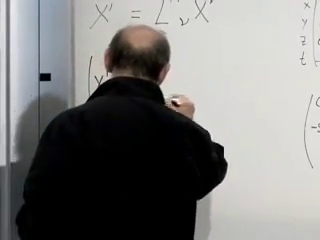
\includegraphics[width=0.8\textwidth]{lecture_06_figure_03.png} \caption{المركبات المضادة للتغاير والمتغايرة، ومصفوفة المترية، وبداية التقلص الثابت.} \lectureframe{00:45:00} \end{figure}

إنزال المؤشر ليس مجرد زخرفة. فهو يجمع الإشارات اللازمة للمعيار الثابت تحت لورنتز: \begin{align}
  A_\mu A^\mu
  &=-(A^1)^2-(A^2)^2-(A^3)^2+(A^0)^2,                    \label{eq:l6-norm}\\
  X_\mu X^\mu
  &=t^2-x^2-y^2-z^2.
\end{align} والتعبير الثاني هو الفاصل الزمكاني الثابت من نقطة الأصل. ولأن \(A^\mu\) يتحول بالطريقة نفسها التي يتحول بها \(X^\mu\)، فإن تقلصه يتمتع بالثبات نفسه.

ويعلّمنا هذا الترميز أيضًا قاعدة مفيدة في ضبط المؤشرات. فمؤشر الجمع المكرر يظهر مرة في الموضع العلوي ومرة في الموضع السفلي. فمثلًا، \begin{equation}
  A_\mu A^\mu
  =\eta_{\mu\nu}A^\mu A^\nu.
\end{equation} ويمكن تغيير أسماء مؤشرات الجمع، أو المؤشرات الصورية، من غير أن تتغير الكمية.

\begin{classroomqa}
\audiencequestion{هل ينبغي اعتبار أحد هذين المتجهين صفًا والآخر عمودًا، وهل يهم ترتيبهما؟}
\lecturerresponse{في هذا الحساب الحالي، اعتبر الكميات ذات الفهارس مركباتٍ ودَعِ المتريّة تُجري الانكماش؛ فلا حاجة إلى تحويل النقاش إلى جبر مؤثرات من نوع صفّ مقابل عمود. فهذه أعداد عادية، ولذلك لا يهم ترتيبها. أما المؤثرات غير المتبادلة فتتطلب مزيدًا من العناية، لكن هذا ليس موضوعنا هنا.}
\end{classroomqa}

ويعطي البناء نفسه جداءً داخليًا بين متجهين رباعيين مختلفين،
\begin{equation}
  A\mathbin{\cdot}B=A_\mu B^\mu=A^\mu B_\mu.
\end{equation}
وتتبع ثباتيته من دون كتابة مصفوفة لورنتز صريحة. وبما أن \(A+B\) و\(A-B\) متجهان رباعيان، فإن مربع معيار كلٍّ منهما ثابت:
\begin{align}
  (A+B)^2&=A^2+B^2+2A\mathbin{\cdot}B,\\
  (A-B)^2&=A^2+B^2-2A\mathbin{\cdot}B.
\end{align}
وبالطرح نحصل على
\begin{equation}
  (A+B)^2-(A-B)^2=4A\mathbin{\cdot}B,                    \label{eq:l6-polarization}
\end{equation}
ومن ثم فإن \(A\mathbin{\cdot}B\) ثابت أيضًا. وينتج العامل أربعة مباشرةً من التوسيع.\editorialnote{تُقدِّم الحجة المعروضة على اللوح هوية الاستقطاب هذه؛ وكتابة العامل صراحةً تجعل الإلغاء المذكور شفهيًا غير ملتبس.}

\begin{figure}[H]
\centering
\includegraphics[width=0.8\textwidth]{lecture_06_figure_04.png}
\caption{المربعان الثابتان المستخدمان لعزل الجداء الداخلي لمتجهين رباعيين مختلفين.}
\lectureframe{00:52:20}
\end{figure}

الكميات الثابتة مكوّنات طبيعية في القوانين الفيزيائية: فهي، بخلاف مركبة منفردة، تحمل القيمة نفسها من إطار مرجعي إلى آخر.

\section{السرعة الخاصة والزخم الرباعي}

لننظر إلى حدثين متجاورين على خط عالم جسيم. فإن الفاصل بينهما هو المتجه الرباعي التفاضلي المتناهي في الصغر
\begin{equation}
  dX^\mu=(dx,dy,dz,dt).
\end{equation}
وبالنسبة إلى خط عالم زمني، يُعرَّف الزمن الخاص بـ
\begin{equation}
  d\tau^2=dX_\mu dX^\mu
  =dt^2-dx^2-dy^2-dz^2.                                  \label{eq:l6-proper-time}
\end{equation}
والسرعة الرباعية الخاصة هي
\begin{equation}
  U^\mu=\frac{dX^\mu}{d\tau}.                            \label{eq:l6-four-velocity}
\end{equation}
وهي تقيس معدل تغيّر موضع الزمكان بالنسبة إلى الزمن الخاص للجسيم نفسه، لا بالنسبة إلى الزمن الإحداثي لإطار مرجعي مختار.

مع أن \(U^\mu\) له أربع مركبات، فإن ثلاثًا فقط منها مستقلة. وبقسمة المعادلة ~\eqref{eq:l6-proper-time} على \(d\tau^2\) نحصل على
\begin{equation}
  U_\mu U^\mu=1.
\end{equation}
ومن ثم فإن السرعة الرباعية متجه زمني معياره واحد. ويحدِّد اختيار الاتجاه نحو المستقبل إشارة مركبته الزمنية.

\begin{classroomqa}
\audiencequestion{عند سرعات أصغر بكثير من \(c\)، هل تؤول السرعة الرباعية إلى السرعة العادية؟}
\lecturerresponse{تقترب مركباتها المكانية الثلاث من السرعة العادية، بينما تقترب مركبتها الزمنية من الواحد في وحدات \(c=1\). وتنتج هذه العلاقة من تطبيق قاعدة السلسلة وحساب \(dt/d\tau\).}
\end{classroomqa}

أما لكل مركبة مكانية، فلدينا
\begin{equation}
  U^i=\frac{dx^i}{d\tau}
     =\frac{dx^i}{dt}\frac{dt}{d\tau}
     =v^i\frac{dt}{d\tau}.
\end{equation}
وبقسمة المعادلة ~\eqref{eq:l6-proper-time} على \(dt^2\) نحصل على:
\begin{equation}
  \left(\frac{d\tau}{dt}\right)^2
  =1-v_x^2-v_y^2-v_z^2
  =1-\boldsymbol v^2.
\end{equation}
ومن ثم
\begin{equation}
  \frac{dt}{d\tau}=\frac{1}{\sqrt{1-\boldsymbol v^2}}
  =\gamma(\lvert\boldsymbol v\rvert),
\end{equation}
و
\begin{equation}
  U^\mu=(\gamma v_x,\gamma v_y,\gamma v_z,\gamma).
                                                                  \label{eq:l6-u-components}
\end{equation}

\begin{figure}[H]
\centering
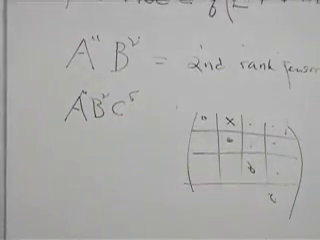
\includegraphics[width=0.8\textwidth]{lecture_06_figure_05.png}
\caption{حساب الزمن الخاص الذي ينتج \(dt/d\tau=\gamma\) ويربط السرعة الخاصة بالسرعة العادية.}
\lectureframe{01:02:00}
\end{figure}

\begin{classroomqa}
\audiencequestion{هل تعني \(dx^2/dt^2\) مشتقةً ثانية، وهل ينبغي أن ينتج عن تربيع متجه حدود مختلطة؟}
\lecturerresponse{هنا تعني \((dx/dt)^2\)، أي مربع مشتقة أولى. وعلاوة على ذلك، تعني \(\boldsymbol v^2\) الجداء النقطي الإقليدي \(v_x^2+v_y^2+v_z^2\)، لا مربع المجموع الصوري \(v_x+v_y+v_z\)؛ ولا توجد حدود مختلطة.}
\end{classroomqa}

\begin{classroomqa}
\audiencequestion{هل تمثل \(v\) في \(\gamma(v)\) السرعة النسبية لإطارين إحداثيين أم سرعة الجسيم؟}
\lecturerresponse{هنا هي سرعة الجسيم في الإطار المختار. ويمكن تقييم الدالة \(\gamma(v)=1/\sqrt{1-v^2}\) عند أي سرعة: ففي تحويل دفعي تُقيَّم عند السرعة النسبية بين الإطارين؛ وفي السرعة الرباعية تُقيَّم عند سرعة الجسيم.}
\end{classroomqa}

عندما يكون \(v\ll1\)، يكون \(\gamma\simeq1\)، لذا تقترب المركبات المكانية لـ \(U^\mu\) من \(\boldsymbol v\) وتقترب \(U^0\) من الواحد. ومع اقتراب السرعة العادية من سرعة الضوء، يزداد \(\gamma\) وجميع المركبات غير الصفرية للسرعة الرباعية بلا حد.

\begin{classroomqa}
\audiencequestion{ألا ينبغي أن تكون لـ \(U^0\) وحدات سرعة بدلًا من أن تكون قريبة من العدد واحد؟}
\lecturerresponse{اختفت الوحدات عندما جُعل \(c\) مساويًا للواحد. ومع \(X^0=ct\)، يكون لدينا
\(U^\mu=(\gamma\boldsymbol v,\gamma c)\)، لذا تقترب المركبة الزمنية من \(c\) ويصبح \(U_\mu U^\mu=c^2\).}
\end{classroomqa}

لجسيم كتلته السكونية \(m\)، نعرّف الزخم الرباعي بـ
\begin{equation}
  P^\mu=mU^\mu.
\end{equation}
في الوحدات الطبيعية،
\begin{equation}
  P^\mu=(\gamma m\boldsymbol v,\gamma m).
\end{equation}
تقترب المركبات الثلاث الأولى من الزخم النيوتني \(m\boldsymbol v\) عند السرعات المنخفضة. وبإعادة الوحدات نحصل على
\begin{equation}
  P^\mu=(\gamma m\boldsymbol v,E/c),
  \qquad E=\gamma mc^2,
\end{equation}
ومن ثم
\begin{equation}
  E=mc^2+\frac{1}{2}m\boldsymbol v^2+O(mv^4/c^2).
\end{equation}
المركبة الزمنية هي الطاقة بوحدات \(c=1\)، أو الطاقة مقسومة على \(c\) عندما تُعطى جميع المركبات الأربع وحدات الزخم.

\begin{classroomqa}
\audiencequestion{هل تكون \(\boldsymbol v\) العادية، مع إلحاق مركبة رابعة بها، متجهًا رباعيًا بحد ذاتها؟}
\lecturerresponse{لا. السرعة الثلاثية العادية لا تتحول كمتجه رباعي. العامل \(\gamma\) وتعريف الزمن الخاص أساسيان؛ فالمتجه الرباعي هو \(U^\mu\)، وليس \(\boldsymbol v\).}
\end{classroomqa}

\section{لماذا يجب أن يختلط المجالان الكهربائي والمغناطيسي}

نأخذ الآن ما سُمّي استراحة قصيرة من النسبية. لنبدأ بمعادلة الحركة ما قبل أينشتاين ونسأل كيف يجب إعادة تنظيمها قبل أن تصبح صالحة في كل إطار قصوري. التسارع العادي هو المشتقة الزمنية للسرعة العادية. ونظيره رباعي الأبعاد هو بطبيعة الحال
\begin{equation}
  A^\mu=\frac{dU^\mu}{d\tau}.
\end{equation}
عند السرعات المنخفضة، تقترب مركباته المكانية من التسارع العادي. سنؤجل المعادلة النسبية الكاملة؛ ولنعاين أولًا قانون القوة القديم.

بالنسبة إلى شحنة \(q\) في مجالين كهربائي ومغناطيسي،
\begin{equation}
  \boldsymbol F=m\boldsymbol a
  =q\left(\boldsymbol E+\boldsymbol v\times\boldsymbol B\right).
                                                                  \label{eq:l6-lorentz-force}
\end{equation}
الحد الكهربائي مستقل عن سرعة الجسيم، في حين أن الحد المغناطيسي ليس كذلك.

\begin{figure}[H]
\centering
\includegraphics[width=0.8\textwidth]{lecture_06_figure_06.png}
\caption{الصيغة ما قبل النسبية لقانون قوة لورنتز التي تحفّز على الجمع بين \(\boldsymbol E\) و\(\boldsymbol B\).}
\lectureframe{01:18:20}
\end{figure}

افترض أن راصدًا لا يرى مجالًا كهربائيًا، لكنه يرى مجالًا مغناطيسيًا وشحنة متحركة. تتعرض الشحنة لقوة مغناطيسية. غير أنه في إطار السكون اللحظي للشحنة، \(\boldsymbol v=0\)، ولذلك ينعدم الحد المغناطيسي في المعادلة~\eqref{eq:l6-lorentz-force}. ولم يصبح خط العالم الفيزيائي قصوريًا لمجرد أن الإحداثيات تغيّرت؛ لذا لا بد أن تشتمل القوة في الإطار الجديد على مساهمة كهربائية. وبصياغة أدق، لا يمكن تحويل تسارع رباعي غير صفري إلى الصفر بمجرد تغيير الأطر القصورية، مع أن التسارع الثلاثي ومركباته يتحولان بالفعل. \editorialnote{تمثل عبارة التسارع الرباعي هذه الصيغة اللامتغيرة للحجة المطروحة في قاعة الدرس، وتتجنب التعامل مع التسارع الثلاثي العادي نفسه على أنه لا يتغير بتغير الإطار.}

وعليه، يجب أن يتحول المجالان الكهربائي والمغناطيسي أحدهما إلى الآخر. ولهما معًا ست مركبات، لذلك فهما ليسا كمية قياسية واحدة ولا متجهًا رباعيًّا واحدًا. نحتاج إلى كائن جديد ذي قانون تحول.

\section{الموترات: تحول واحد لكل فهرس}

يجوز أن تُسمى الكمية القياسية موترًا من الرتبة صفر؛ فهي لا تملك فهارس. والمتجه الرباعي موتر من الرتبة الأولى؛ وله فهرس واحد له أربع قيم ممكنة. وأبسط مثال من الرتبة الثانية هو الجداء
\begin{equation}
  A^\mu B^\nu.
\end{equation}
ولكل فهرس أربع قيم، لذا يملك هذا الكائن \(4^2=16\) مركبة، ويمكن عرضها في هيئة مصفوفة \(4\times4\). أما جداء ثلاثة متجهات،
\begin{equation}
  A^\mu B^\nu C^\sigma,
\end{equation}
فله \(4^3=64\) مركبة، وهو موتر من الرتبة الثالثة. وتستمر الرتب الأعلى على هذا النمط. والاسم أقل أهمية من القاعدة التي تعرّف هذا الكائن.

إذا كان
\begin{equation}
  A'^{\mu}=\Lambda^\mu{}_{\nu}A^\nu,
  \qquad
  B'^{\sigma}=\Lambda^\sigma{}_{\tau}B^\tau,
\end{equation}
فإن جداءهما يتحول على النحو
\begin{equation}
  A'^{\mu}B'^{\sigma}
  =\Lambda^\mu{}_{\nu}\Lambda^\sigma{}_{\tau}
   A^\nu B^\tau.
\end{equation}
وهذا يعطينا القانون التعريفي لموتر مضادّ التغاير من الرتبة الثانية:
\begin{equation}
  T'^{\mu\sigma}
  =\Lambda^\mu{}_{\nu}\Lambda^\sigma{}_{\tau}T^{\nu\tau}.
                                                                  \label{eq:l6-tensor-transform}
\end{equation}
توجد مصفوفة لورنتز واحدة لكل فهرس. ويُجمَع على \(\nu\) و\(\tau\) المكررين؛ أما \(\mu\) و\(\sigma\) الحرّان فيحددان المركبة الجاري حسابها في الإطار المشار إليه بشرطة.

\begin{figure}[H]
\centering
\includegraphics[width=0.82\textwidth]{lecture_06_figure_07.png}
\caption{تحول متجهين، وقانون التحول الناتج ذي المصفوفتين لموتر من الرتبة الثانية.}
\lectureframe{01:27:15}
\end{figure}

لا يشترط أن يكون الموتر جداءً واحدًا لمتجهات. فكل من \(A^\mu B^\nu\) و\(A^\nu B^\mu\) يخضع لقانون تحول الموتر، وكذلك مجموعهما وأي مجموع من قبيل
\begin{equation}
  A^\mu B^\nu+C^\mu D^\nu.
\end{equation}
فقانون التحول، لا تحليل معيّن إلى عوامل، هو التعريف. ويكتسب موتر من الرتبة الثالثة مصفوفة لورنتز ثالثة، وهكذا.

\section{الموترات المتناظرة والمضادة للتناظر}

ستكون فئتان من موترات الرتبة الثانية مفيدتين على نحو خاص. فالموتر المتناظر يحقق
\begin{equation}
  T^{\mu\nu}=T^{\nu\mu},
\end{equation}
بحيث تتطابق العناصر المنعكسة عبر القطر. وتحدد عناصره الأربعة الواقعة على القطر وستة عناصر على أحد جانبي القطر بقية العناصر، فنحصل على
\begin{equation}
  4+6=10
\end{equation}
مركبات مستقلة.

أما الموتر المضاد للتناظر فيحقق
\begin{equation}
  T^{\mu\nu}=-T^{\nu\mu}.                                \label{eq:l6-antisymmetry}
\end{equation}
وبوضع \(\mu=\nu\) في المعادلة~\eqref{eq:l6-antisymmetry} نحصل على
\(T^{\mu\mu}=-T^{\mu\mu}\)، ولذلك ينعدم كل عنصر قطري. وتحدد العناصر الستة في أحد النصفين المثلثيين العناصر الستة الأخرى بتغير في الإشارة. ولذلك توجد بالضبط ست مركبات مستقلة.

\begin{figure}[H]
\centering
\includegraphics[width=0.82\textwidth]{lecture_06_figure_08.png}
\caption{مصفوفة \(4\times4\) مضادّة التناظر مكتملة: أصفار على القطر
وعلامات متعاكسة على جانبيه.}
\lectureframe{01:34:25}
\end{figure}

هذا العدد هو المفتاح. فالمركبات الكهربائية الثلاث والمركبات المغناطيسية الثلاث يمكن أن تنتظم في موتر واحد مضادّ التناظر من الرتبة الثانية.

\section{موتر المجال الكهرومغناطيسي}

لتكن وسوم الزمكان عبر الصفوف والأعمدة بالترتيب
\((1,2,3,0)=(x,y,z,t)\). والترتيب المكتوب على اللوح هو
\begin{equation}
  F_{\mu\nu}=
  \begin{pmatrix}
    0    & -B_3 & B_2  & E_1\\
    B_3  & 0    & -B_1 & E_2\\
    -B_2 & B_1  & 0    & E_3\\
    -E_1 & -E_2 & -E_3 & 0
  \end{pmatrix}.                                         \label{eq:l6-field-tensor}
\end{equation}
تحتوي الخانات المكانية البحتة على المجال المغناطيسي؛ أما الخانات التي تحمل مؤشرًا مكانيًا وآخر زمنيًا فتحتوي على المجال الكهربائي. ويعطي ضدّ التناظر عناصر المثلث السفلي متى عُرفت عناصر المثلث العلوي.

\begin{classroomqa}
\audiencequestion{هل جميع المدخلات المغناطيسية سالبة، وهل تقابل الوسوم
\(x,y,z\)؟}
\lecturerresponse{تتناوب الإشارات في المثلث المكاني العلوي كما هو مبيّن:
\(-B_3,+B_2,-B_1\). والوسوم \(1,2,3\) تقابل \(x,y,z\)، بينما
\(0\) يوسم الزمن. والانعكاس عبر القطر يعكس كل إشارة.}
\end{classroomqa}

\begin{figure}[H]
\centering
\includegraphics[width=0.82\textwidth]{lecture_06_figure_09.png}
\caption{موتر المجال الكهرومغناطيسي بعد اكتماله، وفق ترتيب المركبات الذي يقدّم المكونات المكانية في هذه المحاضرة.}
\lectureframe{01:41:05}
\end{figure}

الاصطلاح المتعارف عليه هو \(F_{\mu\nu}\)، لا الرمز العام
\(T_{\mu\nu}\). ويخمّن المحاضر أن الحرف قد يشير إلى
Faraday، مع تصريحه صراحةً بأنه لا يعرف تاريخ هذا
الاصطلاح. والمهم هنا هو ضدّ تناظره ومركباته الحقلية الست،
لا ذلك التخمين المتعلق بالحرف.

\begin{classroomqa}
\audiencequestion{هل يمثّل كل عنصر في المصفوفة شدةَ مجالٍ في
المستوى الإحداثي المشار إليه؟}
\lecturerresponse{إنه مركبة من موتر المجال الكهرومغناطيسي.
فالعناصر التي تتضمن الزمن هي مركبات كهربائية، والعناصر ذات المؤشرين المكانيين--المكانيين
ترمّز المركبات المغناطيسية.}
\end{classroomqa}

اعزل الصف والعمود اللذين يحملان مؤشر الزمن. والكتلة المتبقية
\(3\times3\) المضادّة للتناظر مغناطيسية. ويمكن تذكّر عناصرها المستقلة
على نحو دوري:
\begin{equation}
  F_{12}=-B_3,
  \qquad F_{23}=-B_1,
  \qquad F_{31}=-B_2.                                   \label{eq:l6-magnetic-cycle}
\end{equation}
وانطلاقًا من العلاقة الأولى، حرّك كل وسم على الدورة
\(1\to2\to3\to1\). وبصورة مكافئة،
\begin{equation}
  F_{ij}=-\epsilon_{ijk}B_k,
\end{equation}
مع \(\epsilon_{123}=+1\).\editorialnote{صيغة Levi--Civita هي
الصيغة القياسية الموجزة للقاعدة الدورية التي فُصّلت صراحةً على اللوح.}

\begin{figure}[H]
\centering
\includegraphics[width=0.82\textwidth]{lecture_06_figure_10.png}
\caption{المركبات المكانية الدورية التي ترمّز المجال المغناطيسي في الموتر
المضادّ للتناظر.}
\lectureframe{01:46:20}
\end{figure}

أما المطابقات الخاصة بالمجال الكهربائي فهي أكثر مباشرةً:
\begin{equation}
  E_1=F_{10},
  \qquad E_2=F_{20},
  \qquad E_3=F_{30}.
\end{equation}

لذلك للمجال المغناطيسي وصفان مفيدان. ففي الفضاء ثلاثي الأبعاد، يمكن إقران متجه محوري ذي ثلاث مركبات بموتر
\(3\times3\) مضادّ للتناظر. أما في الزمكان، فهو ليس إلا الجزء
المكاني من الموتر ذي المركبات الست \(F_{\mu\nu}\). وهذا الإقران
خاص بثلاثة أبعاد: فالموتر المضادّ للتناظر \(4\times4\) له ست
مركبات مستقلة ولا يمكن مطابقته بمتجه رباعي.
\editorialnote{تحت الدورانات الصحيحة يتصرف المجال المغناطيسي كمتجه؛
أما تحت الانعكاسات فهو، على نحو أدق، متجه محوري، أو شبه متجه.}

ليس الغرض من هذا البناء مجرد عدّ المركبات لذاته.
ولأن \(F_{\mu\nu}\) يتحول كموتر، فإن تحويل لورنتز من نوع الدفعة
يمزج تلقائيًا بين عناصره الكهربائية والمغناطيسية. وفي المحاضرة التالية يمكن
ضمّه إلى السرعة الرباعية والتسارع الرباعي لاستبدال
المعادلة ~\eqref{eq:l6-lorentz-force} بمعادلة حركة متغايرة.

\section{أسئلة حول آينشتاين ومينكوفسكي}

تنتقل الدقائق الأخيرة من الصياغة الشكلية إلى الكيفية التي نشأت بها تاريخيًا. وتُطرح الإجابات على أنها استذكارات لا تاريخًا محسومًا، وهذا التحفّظ جزء من التبادل نفسه.

\begin{classroomqa}
\audiencequestion{هل كان آينشتاين يسعى إلى صياغة ثابتة تحت تحولات لورنتز
بدوافع مفهومية، أم أن ملاحظات معيّنة هي التي دفعته؟}
\lecturerresponse{كان المبدأ القائل إن قوانين الطبيعة ينبغي أن تكون لها
الصيغة نفسها في كل إطار قصوري عنصرًا مركزيًا في تفكيره. وكانت هناك أيضًا
أدلة تجريبية تتعلق بالضوء وبالإخفاق في كشف الحركة
عبر الأثير، مع أن المحاضر يصرّح صراحةً بأنه غير واثق من أي
النتائج كان آينشتاين يعرفها، أو من مدى قوة تأثيرها فيه. وكان الضغط
المفهومي هو أن معادلات ماكسويل وقوة لورنتز ينبغي أن تطيع
مبدأ النسبية، وهذا يقتضي أن تتحول الحقول الكهربائية والحقول
المغناطيسية ومركبات السرعة معًا.}
\end{classroomqa}

عرض آينشتاين في 1905 لم يستخدم الصياغة الموجزة بالمتجهات الرباعية
المستخدمة هنا. بل جرى فيه العمل مركبةً بعد مركبة، مع كتابة
العوامل اللازمة من \(\gamma\) والسرعة صراحةً. ثم نظّم مينكوفسكي
البنية نفسها هندسيًا بوصفها زمكانًا رباعي الأبعاد.

\begin{classroomqa}
\audiencequestion{هل قاوم آينشتاين صياغة مينكوفسكي للزمكان،
وبعد كم من الوقت قدّمها مينكوفسكي؟}
\lecturerresponse{الاستذكار المطروح في الصف هو أن آينشتاين لم
يرحّب في البداية باللغة الهندسية رباعية الأبعاد، لكنه تبنّى
قيمتها سريعًا. ويُذكر التوقيت على نحو تحفّظي بأنه بعد ورقة
1905 بنحو سنتين تقريبًا، وربما كان ذلك في 1907؛ ويشدد المتحدث على أنه
يسترجع من الذاكرة لا يثبت التاريخ.}
\end{classroomqa}

\begin{classroomqa}
\audiencequestion{هل كان مينكوفسكي رياضيًا أم فيزيائيًا، وما الذي أسهم به أيضًا،
وهل تأثر بلورنتز أو بفيتزجيرالد؟}
\lecturerresponse{لا يُدَّعى هنا جواب واثق. ولم تُستقصَ مسألة
كونه رياضيًا أم فيزيائيًا، وتقطع مداخلة من الجمهور ملاحظةً عامة
عن أعمال مينكوفسكي الأخرى، وتُترك مسارات التأثير الممكنة غير مؤكدة
صراحةً. والنقطة الموثوقة في هذا النقاش هي تنظيم مينكوفسكي الحاسم
للنسبية في ترميز هندسي رباعي الأبعاد.}
\end{classroomqa}

\begin{classroomqa}
\audiencequestion{هل كانت التحولات التي تمزج \(\boldsymbol E\) و
\(\boldsymbol B\) موجودةً بالفعل في عمل آينشتاين عام 1905؟}
\lecturerresponse{نعم، ولكنها كُتبت مركبةً بعد مركبة لا في معادلة
واحدة لموتر المجال. والمقارنة التي أُجريت في الصف هي مع
معادلات ماكسويل المكتوبة بالمركبات: فقد يكون المضمون حاضرًا قبل الصياغة
الموجزة التي تكشف بنيته المشتركة. وكانت مساهمة مينكوفسكي هي جعل
تلك البنية منهجيةً في لغة الزمكان.}
\end{classroomqa}

وهذا يعيدنا إلى النقطة الرياضية التي بدأنا بها. فالمركبات لا غنى عنها
في الحساب، لكن القانون يصبح مفهومًا عندما تُعرَف تلك المركبات على
أنها أجزاء من كمية واحدة تتحول. والمهمة التالية هي استخدام \(F_{\mu\nu}\) لكتابة
معادلة حركة الجسيم المشحون في صيغة تكون نفسها في
كل إطار قصوري.